\section{Latent Gaussian Process Classifier}

\thispagestyle{empty}
Expanding on the same idea of separate latent GPs for multiple sequences of each trial, in this section we introduce  a new model that combines a logistic classifier with our extended GPBFA model. This  GP based latent classifier for high dimensional temporal instances proves to be an effective classifier since it not only projects the observations into latent space but also learns a discriminatory plane in that space simultaneously.

\subsection{The Model}

In previous sections we studied models that are able to learn the inherent structure from high dimensional instances of observations, in this model we combine the latent model with a classifier and use a variatioanl algorithm to get closer to the optimal distributions one step at a time. 

Consider observations $ {Y,L}$, where $ Y \in \mathcal{R} S \times C \times N$ and each observational instance $Y[s]$ is associated with a label $L, L \in {-1,1} S \times 1$ signifying it to be in one class or another. 

Conceptually one can imagine that  both data and its labels arise from the same latent space. The discriminatory information about the samples (labels) thus, can be further utilized to learn the most relevant latent space, i.e. the one in which data can be separated best.

\begin{figure}
    \centering
    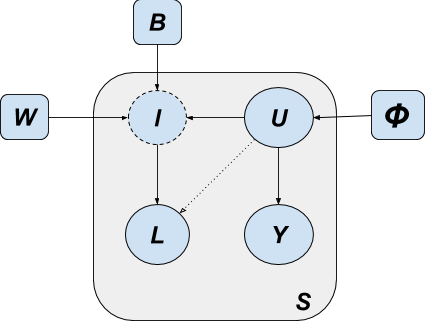
\includegraphics[scale=0.5]{thesis/images/LCMGP_Model.png}
    \caption{Graphical representation of Gaussian Process based latent classifier (lgpc)}
    \label{fig:lgpc}
\end{figure}

As can be seen from figure \ref{fig:lgpc}, 
we introduced a dummy variable $l$  to help  us keep track of classifier values in the latent space. For each data sample $s \in S$, a set of latent processes $u \in U , u \in \mathcal{R}^{P \times N} $ are assumed to generate observed sequence $Y[s] \in \mathcal{R}^{P \times N} $  through mixing matrix $\phi \in \mathcal{R}^{C \times P} $ and a class label $L[s] \in [-1,+1]$. To learn the separation plane in latent space we attach a logistic classifier between $U$ and $L$ such that in additional to $Y, U$ also generates $l  R^1$. Parameters  of classifier are  $W \in R^S$ and a bias term $B$. Values of l then can be converted into class labels through a static rule $ L[s] = \{1 if l[s] > 0,  -1 otherwise\}$. Similar to the model in previous section we vectorize latent and actual observations for computation purposes, making $U \in mathcal{R}^ {S \times CN}, U \in mathcal{R}^ {S \times PN}$, giving the generative model as,




\begin{equation}
Y= U * \bar{\phi}^T + \sigma^2I
\end{equation}

Once again ${  \bar{\phi} = \phi \times I_{N \otimes N} }$ is also a block diagonal of size $CN \times PN$ with $C \times P$ matrix ${\phi}$ on its diagonal. Corresponding latent label values $l$ are generated as, 

\begin{equation}
l= B + U * W^T + s^2I
\end{equation}

and finally the Labels for each data instance  can be generated through the rule {$L[s] = -1$ if $l[s] < \mu L[s] = +1$, otherwise}
Thus combined data gneration model along with priors can be given as,

\begin{equation}
p(W) \approx \mathcal{N}(W \mid 0, I)
\end{equation}
\begin{equation}
p(B) \approx \mathcal{N}(B \mid 0, I)
\end{equation}
\begin{equation}
p(\phi) \approx \mathcal{N}(\phi \mid 0, I)
\end{equation}
\begin{equation}
p(l | U, B, W) \approx \mathcal{N}(l \mid W^{T}U + B, s^2I)
\end{equation}
\begin{equation}
p(L | l) \approx \delta(Ll > \nu)
\end{equation}
Additionally, We put a GP prior on latent variable $ u \in GP(0,\bar{K^p})$ associated with each observational instance where $\bar{K}$ is also a block diagonal of size $PN \times PN$ with co-variance kernels ${K_p \in R ^{N \times N}}$ for each  Gaussian process on diagonals.

Also, just like in previous model we introduce inducing variable $\hat{u} \in \mathcal{R}^{P \times n}$ for latent processes such that  (n < N) to make the GP inference scalabale. $\hat{u}$ has a GP prior as in previous sections. 

We use a variational inference scheme to approximate the posterior $p(W,B,\hat{u},l \mid Y, L)$.

\subsection{Sparse variatioanl approximation in LCGC}

Following inference as sketched in previous sections we introduce variational distribution $q(W,B,l,\hat{u})$ to approximate the posterior. Variational updates for the parameters can be given as,

\begin{equation}
q(\hat{u}) \approx \mathbb{N}(\hat{u} \mid (y\mathbb{E}[\phi] + \mathbb{E}[w]\mathbb{E}[l]\sigma^2 - \mathbb{E}[w]\mathbb{E}[b]\sigma^2){K}_{pNpn}K_{pnpn}^{-1}\Sigma_{u}^{-1}, \hat{\Sigma_{u}^{-1}})
\end{equation}

where $ \hat{\Sigma_{u}} = K_{pnpn}^{-1} + \frac{1}{\sigma^2}{K_{pnpn}^{-1}K_{pnpN}F_uK_{pNpn}K_{pnpn}^{-1}}$ \\
$F_u = \mathbb{E}[\phi^T\phi] + \sigma^2\mathbb{E}[w^Tw] = Var(\phi) + \mathbb{E}[\phi]^T\mathbb{E}[\phi] + Var(w) + \mathbb{E}[w]^T\mathbb{E}[w]$

Using conditional and affine properties of GP we obtain real latent processes as,

\begin{equation}
q(u) \approx \mathbb{N}(\hat{\mu}M, \Sigma_{u|u^{p}} + M\Sigma_{u}M^{T})}
\end{equation}

where $\hat{\mu}_{u}$ is the mean and ${\hat{\Sigma}_{u}}$ variance of $\hat{u}$\\
Also, $\Sigma_{u|u^{p}} = K_{pNpN} - K_{pNpn}K_{pn}^{-1}K_{pnpN}$ and $M = K_{pnpn}^{-1}K_{pNpn}$

Mixing matrix, 
\begin{equation}
q(\phi) \approx \mathbb{N}(\phi \mid (\bar{V}_{\phi} + I)^{-1}\bar{z}_{\phi}, (\bar{V}_{\phi} + I)^{-1})
\end{equation}
where $\bar{V}_{\phi} = \sum_{s}^{S}(<\bar{u}_s><\bar{u}_s>^T$ + I) 
and $\bar{z}_{\phi} = \sum_{s}^{S}<\bar{u}_s>\bar{y}_{s}^T$
such that $x = vec(\bar{x})$ 

label values in the latent space, 
\begin{equation}
q(l_i) \approx \mathbb{T}\mathbb{N}(l_i \mid (\mathbb{E}[w]\mathbb{E}[u] + \mathbb{E}[b], 2*I, l_i < \mu)
\end{equation}
Here $\mathbb{T}\mathbb{N}$ is the truncated normal distribution and $\mu$ the fixed cut off.

Parameter weights for classifier, 

\begin{equation}
q(W) \approx \mathbb{N}(w \mid [F_u+I]^{-1}(\mathbb{E}[u]^T\mathbb{E}[l] - \mathbb{E}[u]^T\mathbb{E}[B]^T,[F_u+I]^{-1})
\end{equation}

where $F_u = \mathbb{E}[U^{T}U]$

Finally the bias term,
\begin{equation}
q(B) \approx \mathbb{N}(B | (\mathbb{E}[l]^T - \mathbb{E}[U]\mathbb{E}[W]^T,I)
\end{equation}

Derivation details of these approximations can be found in Appendix B. 

\subsection{Prediction using LCGC:}
\begin{figure}
    \centering
    \includegraphics[scale=0.75]{thesis/images/LCGC_input.png}
    \caption{Top: Few sample latent processes (red: negative cases, blue: positive) and mixing matrix, Bottom: Resultant output samples from corresponding processes}
    \label{fig:lcpc_input_demo}
\end{figure}

Category prediction for a new observation follows standard GP prediction steps.
For a new data observation Y*, first we project it to the latent space using \ref{eqn:lcgc_latent}.l* in the latent space can be found using predetermined values of weight parameter and bias. Finally, the label L* can be predicted using static rule for $p(L* \mid l*)$ mentioned in \ref{eqn:LCGC_Lgivenl}. However, since we do not know the values in latent space in advance we have to drop all the terms dependent on them form the expressions.

\begin{equation}
q(u^*) \approx \mathbb{N}(u^* \mid (Y^*\mathbb{E}[\phi])K_{pNpn}K_{pnpn}^{-1}\Sigma_{u}^{-1}M, M\Sigma_{u}M^T)
\end{equation}

\begin{equation}
q(l^*) \approx \mathbb{TN}(l^* \mid (Y^*\mathbb{E}[\phi])K_{pNpn}K_{pnpn}^{-1}\Sigma_{u}^{-1}M, M\Sigma_{u}M^T)
\end{equation}

This also means that some information is lost during prediction and hence it might not be as efficient.



\subsection{Demonstration using LCGC}
For demonstration purposes we use an artificial dataset in which our positive classes are genrated through a special latent process that's a combination of linear and gaussian kernels. This gives us a sort of linear trend. Latent processes for the negative classes are generated using simple gaussian kernels. We pass these through a randomly generated mixing matrix to obtain the observation Y and their corresponding labels L (Figure: \ref{fig:lcpc_input_demo}). 
The observations are then split into training data $(Y_train,L_train)$ and test data $(Y^*,L^*)$. 

\begin{figure}
    \centering
    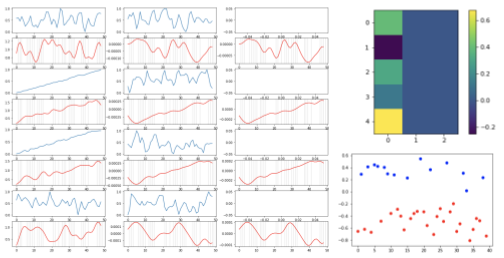
\includegraphics[scale=0.75]{thesis/images/LCGC_output_demo.png}
    \caption{Left: Actual(blue)and extracted(red) latent processes from observed data (vertical lines shows the position of inducing points), Right : Extracted mixing matrix and intermediary variable results on test set}
    \label{fig:lcpc_output_demo}
\end{figure}

To make the inference simple, we used only Gaussian kernel in our GP priors with signal noise ($\sigma = 1$). Figure contains the few extracted latent processes for visual inspection, though we use only $60$ percent of data, we can see that model is able to extract linear trend from the samples. The Gaussian processes are generally ignored due to our assumption of noise to be 1 ($\sigma^2 = 1$), which is also the scale of our observed values. Figure \ref{fig:lcpc_output_demo} also shows the separation of training data in latent space. As can be observed, model is able to achieve a good enough separation of test data in latent space. 















